\section{Sektionsüberschrift}
\label{sec:Anochmalsektion}
\textcolor{red}{!!! Hinweis !!!: Anhänge werden als \textbackslash section definiert.}\\
%
Literatur \cite{DIN3990} \cite{testweb}
%
%===================
\subsection{Subsektion}
\label{sec:Asubsektion}
%
\begin{figure}
	\centering
	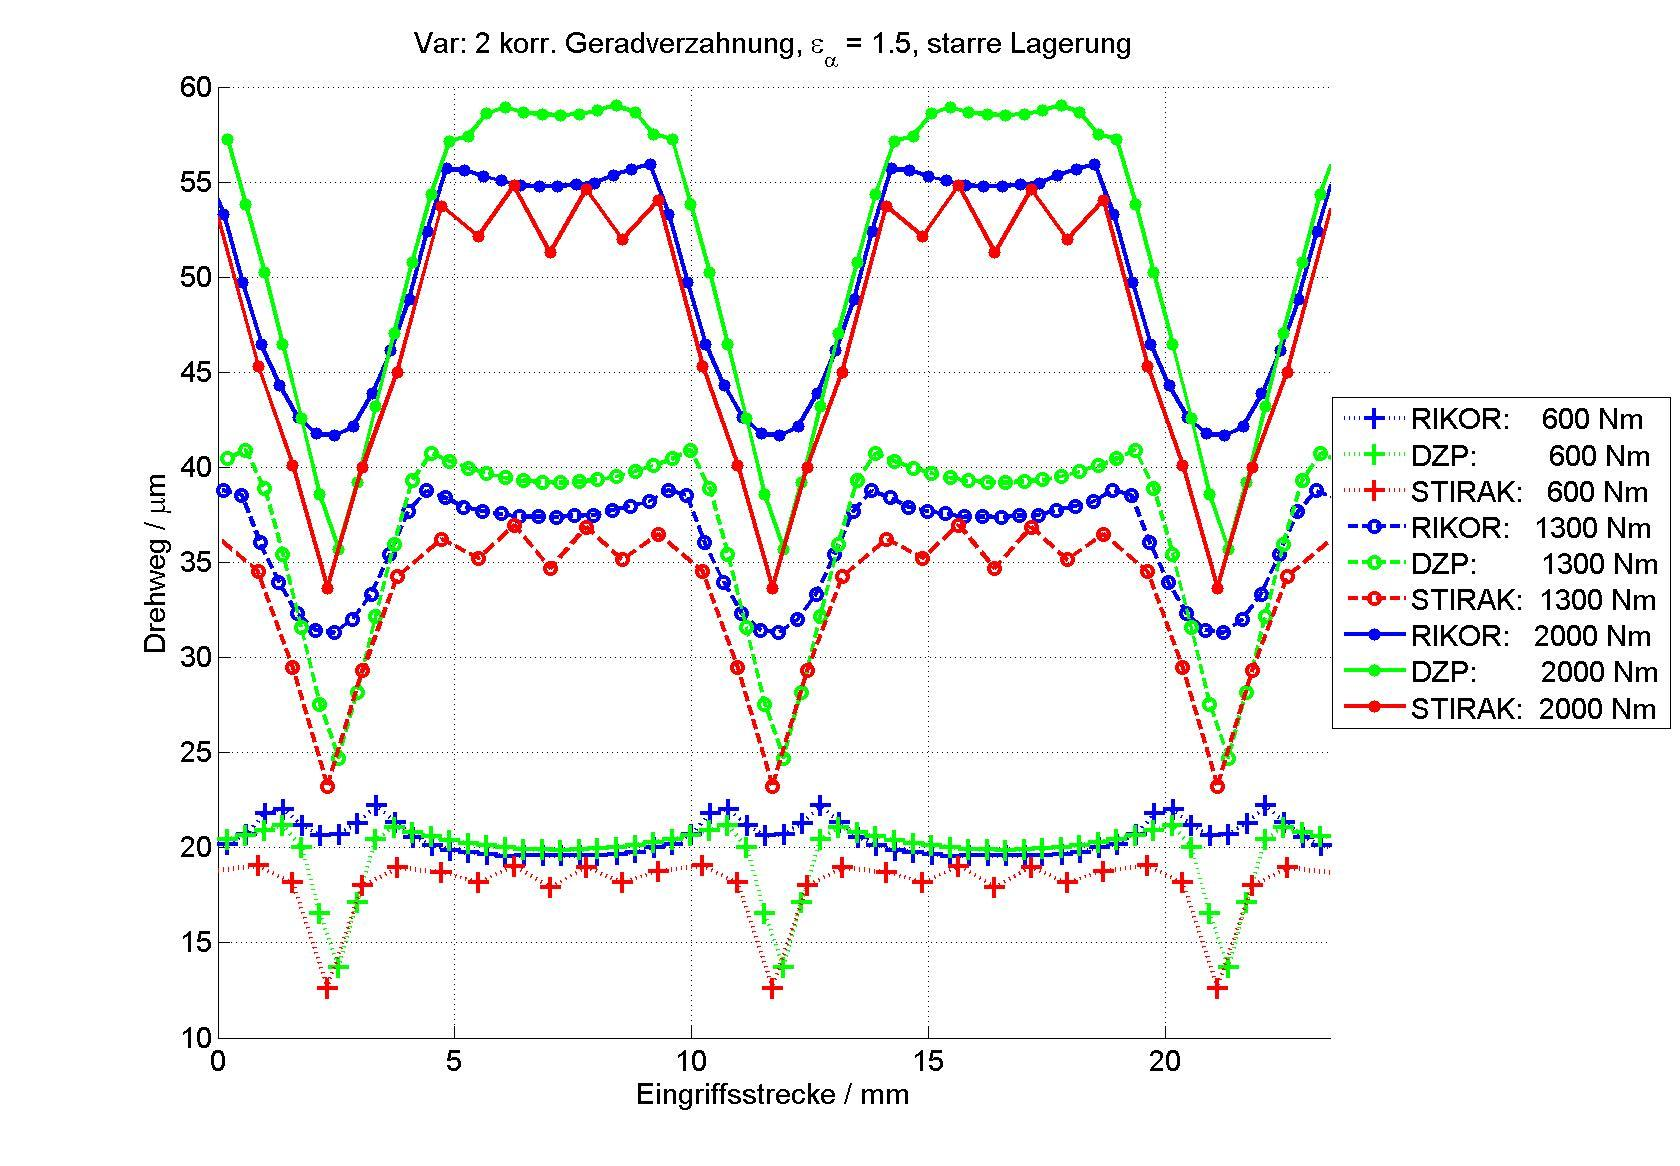
\includegraphics[width=0.5\textwidth]{_ltx/Beispiel.jpg}
	\caption{Dies ist ein wunderschönes Bild, das auch aus einer Quelle und so weiter stammen kann \cite{Niemann01}. Deshalb sind Bildunterschriften so einfach möglich.}
	\label{fig:Abeispiel}
\end{figure}
%
%----------------------
\subsubsection{Subsubsektion}
\label{sec:Asubsubsektion}
%
\textbf{fett} \textit{italic} \textsl{sl} \textsc{Kapitälchen}\\
Formel im Text $\varepsilon$ bla
\begin{equation}
	a^2 + b^2 = c^2
	\label{eq:pytagoras}
	\end{equation}
%
\begin{Gleichungsparameter}
\Gleichungparaeintrag{a}{ - }{Ankathete}{b}{ - }{Gegenkathete}  
\Gleichungparaeintrageinfach{c}{ - }{Hypotenuse}
\end{Gleichungsparameter}
%
%---------
\paragraph{Paragraph}
\label{sec:paragraph}
%
\begin{equation}
	\eta = \dfrac{P_{Ab}}{P_{An}} = \dfrac{P_{An}-P_{V}}{P_{An}}
\end{equation}
%
\begin{Gleichungsparameter}
\Gleichungparaeintrag{\eta}{ - }{Wirkungsgrad}{P_{Ab}}{ kW }{Abtriebsleistung}  
\Gleichungparaeintrag{P_{An}}{ kW }{Antriebsleistung, die auch einen Zeilenumbruch erlaubt}{P_V}{ kW }{Verlustleistung} 
\end{Gleichungsparameter}

Wie man in \eqref{eq:pytagoras} sieht, bzw wie man in \seqref{eq:pytagoras}

\begin{table}
\caption{test}
\end{table}

%---------
\paragraph{Paragraph}
\label{sec:paragraph}
%
\begin{equation}
	\eta = \dfrac{P_{Ab}}{P_{An}} = \dfrac{P_{An}-P_{V}}{P_{An}}
\end{equation}
%
\begin{Gleichungsparameter}
\Gleichungparaeintrag{\eta}{ - }{Wirkungsgrad}{P_{Ab}}{ kW }{Abtriebsleistung}  
\Gleichungparaeintrag{P_{An}}{ kW }{Antriebsleistung, die auch einen Zeilenumbruch erlaubt}{P_V}{ kW }{Verlustleistung} 
\end{Gleichungsparameter}

Wie man in \eqref{eq:pytagoras} sieht, bzw wie man in \seqref{eq:pytagoras}

